\chapter{使用蒙特卡洛方法进行探测器背景模拟}
\label{chapter:background}

为了寻找NLDBD这个极其稀有的事件,一个极低本底的探测环境是PandaXIII实验需要着重解决的问题。所以为了能够在探测器实际建造之前细致的研究探测器结构和材料对本底水平的研究,我们使用Geant4\supercite{Agostinelli:2002hh}作为主要的蒙特卡洛模拟框架,构建了模拟器的模型。通过这个模型我们可以细致的研究探测器各个组件以及环境对实验本底的贡献,并根据这些数据来调节探测器的各种各样参数以达成实验的设计目标。具体的模拟细节如下列小节所述。

\section{目标元素及模拟工具}

因为探测器的铜壁相对较厚,而且铜壁的材料可以制作的较为纯净,在考虑到铜壁的屏蔽效应后,来自铜壁外的$\alpha$射线和$\beta$射线基本不可能到达探测器内部的灵敏区域,所以需要主要考虑到的本底辐射为探测器铜壁内部原件的各种辐射以及环境和材料中的$\gamma$射线。因为$^{136}$Xe的NLDBD事件释放出来的总能量$Q_{\beta\beta}=2458$keV,探测器设计的相对能量分辨率是3\%FWHW(半高全宽),因而我们定义能量窗口($Q_{\beta\beta}-2\sigma$, $Q_{\beta\beta}+2\sigma$)为能量敏感区域(Region Of Interest, ROI),其中$\sigma$为探测器在$Q_{\beta\beta}$处的绝对能量分辨率。计算可得ROI范围为2395keV到2520keV,所以衰变能量落在这个能量范围附近的元素便是我们感兴趣的元素。

根据各种放射性元素的衰变能量和在自然界中的丰度,再结合既往有关$^{136}$Xe的
NLDBD实验研究结果可以得到,我们关心的主要本底来自于$^{214}$Bi的gamma衰变,其能量为2447.8keV,以及来自于$^{208}$Tl的gamma衰变,其能量为2615.keV。这两种元素分别属于$^{238}$U和$^{232}Th$的衰变链中,而这两种放射性元素在自然界中大量的存在,绝大多数的材料都或多或少的含有它们。除了这两种元素,$^{60}$Co可能会释放出1.33MeV和
1.17MeV的$\gamma$射线,虽然两者和能量约为2.5MeV,但是这两个射线相对独立,同时落在探测器敏感区域内的概率不大,在加上读出窗口的限制$^{60}$Co对实验的影响会变得更小,因而在后续的模拟中它并没有被着重研究。表\ref{tab:activities}给出了构建探测器的原料中Th,U的放射性活度。
\renewcommand\arraystretch{1.4}
\begin{table*}[tbh]
    \centering
    \begin{tabular*}{0.75\textwidth}{@{\extracolsep{\fill}}cccc}
        \hline
        \hline
        \multirow{2}{*}{\textbf{材料}} & \multicolumn{3}{c}{\textbf{放射性活度 ($\mu$Bq/kg)}}\\
            & $^{232}$Th & $^{238}$U  & $^{60}$Co \\ \hline
        铜      & 0.2        &   0.75     &     100     \\
        PTFE    & 0.1        &   4.94      &    -      \\
        不锈钢  & 0.32$\times$10$^3$          &    0.5$\times$10$^3$      &     2.6$\times$10$^3$     \\
        超纯水  & 0.04          &     0.12      &     -     \\
        混泥土  & 9.9$\times$10$^6$          &    4.4$\times$10$^6$   &    -    \\
        \hline
        \hline
    \end{tabular*}
    \caption{不同材料的放射性活度表。铜和PTFE的活动数据来自于文献\cite{Abgrall:2016cct},不锈钢的数据来自于文献\cite{LZ_CDR},超纯水的数据来自于PandaXIII的中期报告\cite{cdr},混泥土的数据来自于文献\cite{Zeng2014}。}
    \label{tab:activities}
  \end{table*}
  

PandaXIII模拟工作中我们使用了Geant4软件作为蒙特卡洛模拟框架。Geant4是由
CERN开发的基于C++的蒙特卡罗应用包,它主要用于模拟粒子在物质中发生的各种物理过程。它内置了做粒子追踪所需要的完整方法包括径迹追踪,探测器几何构建,物理模型和数据等等,其中物理过程中包含了极大能量尺度下各种粒子之间的相互作用,材料和元素的数据。该软件被广泛的应用在了核物理,高能物理,医学研究等等领域。

PandaXIII实验在Geant4软件框架的基础上二次开发了两个模拟框架以满足复杂的模拟需求,分别被称作BambooMC和RestG4。BambooMC是由上海交通大学基于
PandaXII暗物质实验的模拟需求开发改进而成,后者是REST软件\supercite{tomas2013development}的一个模块。我们使用这两种框架独立进行了背景模拟工作,并对两者的结果做了交叉检查以确保结果的正确性。本文中的模拟工作都是由BambooMC模拟框架完成的。

\section{探测器结构及本底来源}
\begin{figure}[tbh]
    \centering
    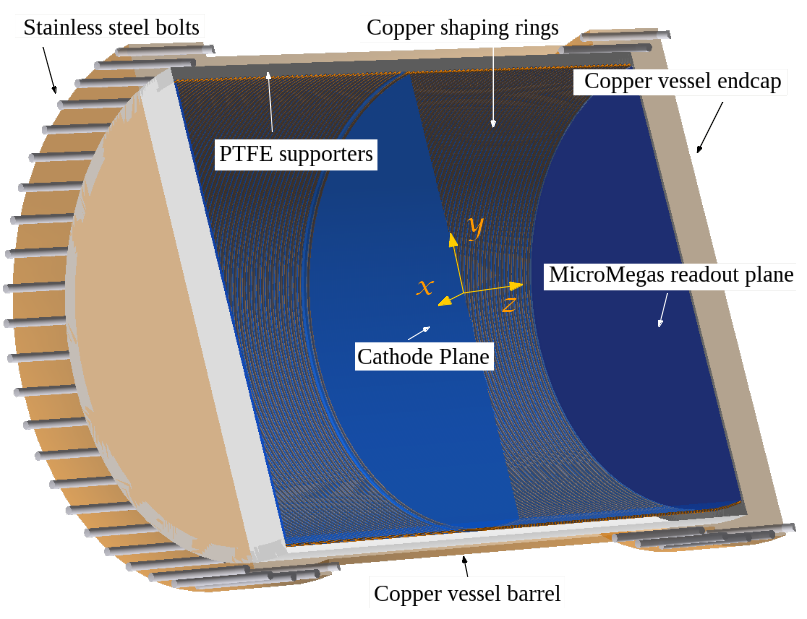
\includegraphics[width=0.4\columnwidth]{pic/fig3.png}
    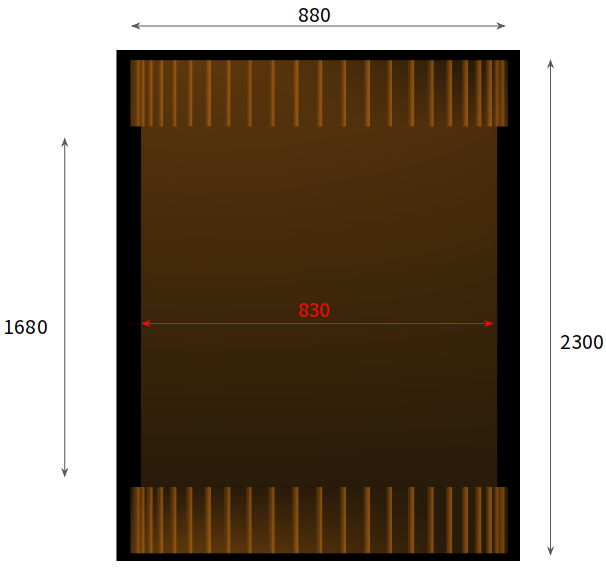
\includegraphics[width=0.4\columnwidth]{pic/fig5.png}
    \caption{左图:Geant4中PandaXIII背景模拟时间漂移室示意图\supercite{cnn},探测器被演奏平面切开。右图:铜罐结构的正视图以及外围尺寸。}
    \label{fig:detector_bamboomc}
\end{figure}

使用BambooMC构建出来的探测器结构如图\ref{fig:detector_bamboomc}所示。铜罐是由一个有法兰的圆柱体和两端的铜盖组成,每侧的铜盖和铜罐之间使用48个不锈钢螺钉铆和,铜罐壁厚度为3厘米,两端铜盖厚度为15厘米。在铜罐内部就是时间漂移室的主体结构,是由5cm厚度PTFE材料的作为支撑,延Z方向镶嵌99个管状圆形铜环组成的场笼,用于形成均匀的延Z方向的漂移电场。两个Micromegas读出平面放置在探测器的两端,同时中心的圆形铜极板将探测器分为上下两个漂移室。探测器主要原件的尺寸可以参照表\ref{tab:parameters_geometry}。
\begin{table*}[thb]
    \begin{center}
        \begin{tabular*}{0.75\textwidth}{@{\extracolsep{\fill}}ccccc}
        \hline
        \hline
        \textbf{组件} & \textbf{参数} & \textbf{值} & \textbf{材料} & \textbf{质量} \\ \hline
        \multirow{3}{*}{铜罐} 
            & 内径 & 80\,cm & \multirow{3}{*}{铜} & \multirow{3}{*}{3438 kg} \\
            & 高度 & 200\,cm &  &    \\   
            & 壁厚 & 3\,cm &  &    \\\hline
        \multirow{2}{*}{铜盖} 
            & 直径 & 88\,cm & \multirow{2}{*}{铜} & \multirow{2}{*}{3320 kg} \\
            & 厚度 & 15\,cm &  &    \\\hline
        \multirow{2}{*}{螺钉} 
            & 直径 & 1.4\,cm & \multirow{2}{*}{不锈钢} & \multirow{2}{*}{230.1 kg} \\
            & 高度 & 40\,cm &  &    \\\hline
        \multirow{4}{*}{场笼} 
            & 内径 & 75\,cm & \multirow{3}{*}{PTFE} & \multirow{3}{*}{1042 kg} \\
            & 高度 & 200\,cm &  & \\ 
            & 厚度 & 5\,cm &  & \\ 
            & 铜环个数 & 99 &    \multirow{1}{*}{铜}  & 118.2 kg \\\hline
        中心极板 
            & 厚度   &   50\,$\mu$m     &   \multirow{1}{*}{铜}  &    0.79 kg   \\   
        \hline
        \hline
        \end{tabular*}
        \caption{探测器组成部件的几何参数,材料以及质量表。\supercite{cdr}}
        \label{tab:parameters_geometry}
    \end{center}
\end{table*}
  
探测器铜罐内填充了200kg的氙气与TMA混合气体,总体气压为10bar,被放置在中国锦屏地下实验室中的水池中。下列详细描述了探测器各个部分对本底的贡献:

\begin{description}
    \item[铜罐] 在模拟中我们将罐体和铜盖一起组成的压力铜罐容器作为了一个整体。虽然电解铜相对洁净(radiopure),但是它作为接近探测气体中最重的组件所产生的背景贡献不可忽略。模拟中使用的铜材料元素活度来自于表\ref{tab:activities}。
    \item[电子学] 因为大多数的电子学器件不可能做的相对洁净,电子学部分产生的本底辐射需要着重考虑,所以在实验的探测器设计中电子学部分被放置在15厘米厚的铜盖外侧以降低其对探测器的影响。在模拟中我们认为电子学$^{238}$U和$^{232}$Th的活度分别为0.26Bq和0.07Bq。此数据是来自于PandaXII暗物质实验的测量结果。
    \item[场笼]场笼是由5厘米厚的PTFE支撑以及等距嵌入的圆环做成的。整个场笼是探测器中质量使用更为仅次与铜罐的组件,其材料的放射性洁净也需要着重考虑,模拟中使用的数据参照表\ref{tab:activities}
    \item[不锈钢螺钉]在组合铜罐时我们使用了96个不锈钢螺丝钉。从表\ref{tab:activities}中可以看不锈钢的放射性洁净程度远远低于其他低本底材料,其活度比铜高了3个量级,因次虽然螺钉的整体质量相对较小,其对本底依然可能造成很大的影响。在模拟中不锈钢螺钉被简化为圆柱体以加速模拟的进行。
    \item[水池中的水]超纯水的放射性相对较低,同时因为水的自屏蔽现象,在模拟中我们只考虑了探测器周围5米范围内的衰变事件。
    \item[实验室水泥墙壁]从表\ref{tab:activities}可以看出水泥自身的放射性比铜高了6个量级,虽然探测器使用了水池来屏蔽,但我们依然需要通过模拟给出水池的最小尺寸以确保水泥及周边环境不会对实验造成过大影响。因为探测器和实验室墙壁之间有着$13\times11\times11$的水池作屏蔽,如果直接模拟水泥墙壁中$^{238}$U和$^{232}$Th的衰变,那么因为模拟效率和模拟数量的限制,基本上不可能有射线能够通过水池达到探测器,所以我们使用了下列的方式来估计实验室水泥墙壁的本底贡献:
    \begin{itemize}
        \item 第一步,我们模拟了在一块巨大的水泥块表面,由水泥内部$^{238}$U和$^{232}$Th产生的$\gamma$射线流的能谱。
        \item 第二步,我们将整个水池分为若干层,逐层的模拟。即根据上一步模拟得到的$\gamma$射线流的能谱,在第一层水的外表面均匀放置$\gamma$粒子,模拟得到穿过这一层水达到内表面的$\gamma$粒子的能谱,方向分布以及数目。随后在第二层的外表面根据第一层得到的粒子能谱和方向分布放置$\gamma$粒子,重复上述模拟过程。假设在第$i$层我们模拟了$N_i$个事件,只有$n_i$个穿过了水池被我们所记录,很容易得到$n_i<<N_i$。那么我们就可以定义$\alpha_i=N_{i+1}/n_i$为放大系数。即在第最后一层我们得到的模拟结果等价于我们不分层直接模拟$N_{eq}$个粒子,其中$$N_{eq}=N_0\Pi_{i=1}{t}a_i$$。其中$N_0$为起始模拟的粒子数目,t为总层数。
        \item 第三步,我们利用上一步中得到的最内层(约$2.5\times2.5\times2.5m^3$)的$\gamma$流能谱和方向分部信息,模拟并统计最终到达探测器内部气体的事件数目和能量分布,并由此计算总体对探测器本底的贡献。
    \end{itemize}
    在上述一层一层迭代的模拟过程中,因为我们关注的能量范围是2457.83keV,因而小于2.2MeV的能谱信息都会被直接忽略,这样可以大大加快计算的速度。
    \item[读出平面]PandaXIII实验中使用了Microbulk MicroMegas读出技术。而这种读出板自身是由低本底的铜以及Kapton塑料制造的。根据相关的实验测量数据,这种读出平面的
    $^{238}$U和$^{232}$Th的放射性约为$45nBq/cm^2$和$14nBq/cm^2$。
    \item[极板]探测器的极板是有铜制作的,而且它质量相对教轻,因次由它自身产生的放射性很低。但是气氙中所含有的部分$^{222}$Rn杂质有可能在电场的作用下富集到极板上,其衰变产物$^{214}$Bi会带来一定的背景信号。在模拟中我们假设Rn的含量为$1mBq/m^3$,即会造成基板上产生约$2nBq/cm^2$的$^{214}$Bi衰变。
\end{description}

我们使用BambooMC模拟框架模拟了上述各种组件对背景的贡献,蒙特卡洛模拟过程中,除了实验室水泥墙外其他组件是将待模拟的元素均匀的放置在结构中或表面上来作为初始粒子(primary particle),即模拟了元素的整个衰变过程,直到达到稳定元素为止。BambooMC模拟使用的物理过程是一个十分简答的考虑了衰变,电磁作用等物理过程,其启用了的模块如下:
\begin{itemize}
    \item G4EmLivermorePhysics
    \item G4EmExtraPhysics
    \item G4DecayPhysics
    \item G4RadioactiveDecayPhysics
    \item G4HadronElasticPhysicsHP
    \item HadronPhysicsShielding
    \item G4HadronPhysicsShielding
    \item G4StoppingPhysics
    \item G4IonQMDPhysics     
\end{itemize}
BambooMC框架会记录每个事件沉积在气体中的hit的能量,位置,发生的物理过程等等相关信息,方便后续的数据分析。在探测器组件背景贡献的相关模拟中,我们主要关心的是探测器接收到的总沉积能量,即总沉积能量在$Q_{\beta\beta}\pm3\%$附近的事件个数就即为产生的背景信号。

在数据处理的过程中还需要注意一点,因为我们的模拟是全链模拟,即一次模拟事件实际上会发生很多次衰变,而且其之间的时间间隔可能会非常的长,因而需要依据事件中各个hit的时间信息进行合理的划分。最终得到的数据如表\ref{tab:rawBck}所示。表中BI是指本底水平(Background Index),用于表示探测器的洁净程度以及屏蔽环境噪声的能力,模拟过程中其计算过程为:
\begin{equation}
    BI = \frac{N_{cpy}}{m_{gas}E_{r}}
    \label{eq:bi}
\end{equation}
其中$N_{cpy}$是指每年探测到的事件数目,$m_{gas}$指探测气体的质量即为200kg,$E_{r}$指ROI的宽度即125.2KeV。

\begin{table*}
    \centering
    \begin{tabular*}{\textwidth}{@{\extracolsep{\fill}}lcccc}
        \hline
        \hline
        \textbf{组件}&\textbf{元素}&\textbf{放射性活度}&\textbf{\multirow{2}{5em}{\centering 本底计数\\计数/年}}&\textbf{ \multirow{2}{8em}{\centering BI\\$10^{-5}c\/(keV\cdot kg\cdot y$)}}\\\\
        \hline
        \multirow{2}{8em}{实验室水泥墙壁\\Laboratory walls}
            & $^{238}$U  &  9.9 Bq/kg & $<0.40\pm0.03$  & -  \\
            & $^{232}$Th &  4.4 Bq/kg &  $<0.22\pm0.02$  & - \\ \hline
        \multirow{2}{8em}{水池\\Water} 
            & $^{238}$U  & 0.12 $\mu$Bq/kg & 0.20 $\pm$ 0.1 &  0.74  \\
            & $^{232}$Th & 0.04 $\mu$Bq/kg & 0.24  $\pm$ 0.06 & 0.96 \\ \hline
        \multirow{3}{8em}{铜罐罐体\\Barrel}
            & $^{238}$U  &  0.75 $\mu$Bq/kg & 1.73  $\pm$ 0.12 &  6.9  \\
            & $^{232}$Th & 0.2  $\mu$Bq/kg & 4.63  $\pm$ 0.18 & 18.5 \\
            & $^{60}$Co  & 10 $\mu$Bq/kg & 9.8  $\pm$ 1.0 &  39.0  \\ \hline
        \multirow{3}{8em}{铜罐盖子\\Endcaps}
            & $^{238}$U  & 0.75 $\mu$Bq/kg  & 0.83  $\pm$ 0.11 &  3.3 \\
            & $^{232}$Th & 0.2 $\mu$Bq/kg & 2.4  $\pm$ 0.1 &  9.8 \\
            & $^{60}$Co  & 10 $\mu$Bq/kg & 4.4  $\pm$ 1.0 &  17.8  \\ \hline
        \multirow{2}{8em}{不锈钢螺钉\\Bolts}              
            & $^{238}$U   &  0.5 mBq/kg & 7.5 $\pm$ 1.5 & 30.1  \\
            & $^{232}$Th  & 0.32 mBq/kg & 39.8 $\pm$ 2.7 & 159  \\ \hline
        \multirow{2}{8em}{场笼支撑体\\Field insulator}    
            & $^{238}$U   & 4.94 $\mu$Bq/kg  & 15.0  $\pm$ 0.5  & 59.9 \\
            & $^{232}$Th  & 0.1 $\mu$Bq/kg & 2.69 $\pm$ 0.03 & 10.7  \\
        \multirow{2}{8em}{铜环\\ Rings}          
            & $^{238}$U  & 0.75 $\mu$Bq/kg  &  0.67 $\pm$ 0.01  & 2.7  \\
            & $^{232}$Th  & 0.2 $\mu$Bq/kg & 0.95 $\pm$ 0.01 &  3.8  \\ \hline
        \multirow{2}{8em}{电子学\\Electronics}
            & $^{238}$U  & 0.26 Bq & 1.0 $\pm$ 0.3  & 4.2  \\
            & $^{232}$Th  & 0.07 Bq & 2.8 $\pm$ 0.2  & 11.3 \\ \hline
        \multirow{2}{8em}{读出平面\\Micromegas}
            & $^{238}$U  & 45 nBq/cm$^2$ & 60.5 $\pm$ 1.7 &  241.6  \\
            & $^{232}$Th  & 14 nBq/cm$^2$ & 23.5 $\pm$ 0.6 &  93.9   \\ \hline
        \multirow{1}{8em}{极板 Cathode}
            & $^{214}$Bi  & 2 nBq/cm$^2$ & 4.1  $\pm$ 0.2  & 16.5 \\
        \hline
        \hline
    \end{tabular*}
    \caption{探测器不同组件对背景信号的贡献,能量区间为2395keV到2520keV。表中的BI是指本底水平(Background Index),关于BI的详细计算过程参见公式\ref{eq:bi}。}
    \label{tab:rawBck}
  \end{table*}
  
从表中可以看出来自与Micromegas的本底辐射是最高的,这是可以理解的。因为Micromegas自身在探测器内部,紧贴着氙气,而且它的放射性活度也相当的大,来自于Micromegas的活度约为$1.59\times10^{-3}$Bq($^{238}$U),相当于7吨重的铜罐的1/6,因而其贡献了相当部分的背景辐射。随后贡献较大的是不锈钢螺钉,虽然它们都在铜罐外面,部分辐射被铜罐所屏蔽,但是不锈钢材料自身的辐射水平太高,其对实验的影响也是相当巨大。

图\ref{fig:stacked_spectrum}使用层叠方式绘制了探测器不同组件所贡献的本底事件能谱分布,能谱范围是2200keV到2700keV,我们需要关注的ROI,即$Q_{\beta\beta}\pm3\% FWHM$为2395keV到2520keV。

\begin{figure}[tbh]
    \centering
    \includegraphics[width=0.4\columnwidth]{pic/fig6.pdf}
    \includegraphics[width=0.4\columnwidth]{pic/fig7.pdf}
    \caption{探测器不同组件所贡献的本底事件能谱分布,能谱范围为2200keV到2700keV,ROI范围为2395keV到2520keV。左图为来自元素$^{238}$U,右图为来自元素$^{232}$Th,两图都为堆叠方式绘制,图例与中文的对应可以参照表\ref{tab:rawBck}。}
    \label{fig:stacked_spectrum}
\end{figure}

\section{探测器响应,读出系统以及电子学触发}

在上述模拟中,我们只考虑到了背景事件在探测器内部沉积的所有能量,并没有考虑到探测器自身的响应以及读出系统带来的影响。举例而言上节模拟中来自于铜罐体$^{60}$Co的背景辐射强度也是相对较大的,因为$^{60}$Co自身会放射出1.33MeV和1.17MeV的两个$\gamma$粒子,如果这两个粒子都被探测器探测到接受那么就有可能收集到一个总沉积能量在$Q_{\beta\beta}$附近的事件。然而这两个$\gamma$粒子之间是完全独立的,哪怕它们同时在探测器内沉积能量,但是它们发生康普顿散射的位置是完全无关的,激发出的电子漂移到读出板的时间也是有间隔的。因而在考虑到探测器的触发过程后,来自$^{60}$Co的本底事件会被极大的压低。本节将会细致的描述和讨论PandaXIII实验模拟过程中对探测器响应以及电子学触发等方面的处理细节。

\subsection{探测器响应}

通过BambooMC的模拟我们可以轻易的得到一个事件在灵敏区域(气氙)内各个hit的相关信息,包括位置,动量,沉积的能量,发生的物理过程等等。在考虑探测器相应的过程中,我们除了需要关注于事件整体沉积能量外,也需要考虑到每个hit的能量大小,并由此模拟电离电子的漂移过程。

探测器时间漂移室被极板分割成了上下两个部分,被入射$\gamma$粒子激发的电子在电场的作用下漂移到探测器两端并被Micromegas收集读出。我们通过Garfield\supercite{garfield}以及
Magboltz\supercite{magboltz}两个软件计算得到了电子在10bar压强的气氙+1\%TMA混合气体中的漂移速度为$v=1.87mm/\mu s$,横向(垂直电场方向)扩散速度(transverse diffusion)为$d _{t}=1.02\times 10^{-2}cm^{1/2}$,纵向(延电场方向)扩散速度(longitudinal diffusion)为$d _{l}=1.39\times 10^{-2}cm^{1/2}$。还有根据之前的文献研究,我们认为该混合气体的电离效率(W Value)为$W=21.9eV$,对应的法诺系数(Fano factor)为$F=0.14$\supercite{Aprile:2009dv}。

我们使用了相对简单的方式来模拟探测器响应:
\begin{enumerate}
    \item 对于BambooMC模拟得到的每个hit,根据hit能量的大小,气体电离效率$W$和法诺系数$F$,利用高斯抽样得到该hit产生的电子数目。
    \item 对于上一步产生的每一个电子,依据它距极板的位置$\Delta z$,计算出横向扩散和纵向扩散的方差,即$\sigma_{t}=d_t*\sqrt{\Delta z}$,$\sigma_{l}=d_l*\sqrt{\Delta z}$。并由此使用高斯采样得到实际的横向扩散距离$s_t$以及纵向扩散距离$s_l$。
    \item 最后就可以根据漂移速度$v$计算得到每个电子真正到达极板的事件和位置信息。
\end{enumerate}
这样我们就将BambooMC模拟得到的每个事件hit的信息转换为了读出平面读出的电子信息,用于接下来的处理过程。

\subsection{电子学触发}
为了合理的设计电子学触发的相关参数,我们使用BambooMC模拟了NLDBD事件产生的两个电子在探测器中的行为(参见章节\ref{chapter:cnn}),统计得到NLDBD事件在气体中绝大部分径迹的尺寸不超过10x10x10$cm^3$,考虑到电子漂移速度,NLDBD事件被读出平面完全收集需要大约$t=10 cm /(1.87 mm/ \mu s) = 53.4\mu s$。我们使用的读出系统对于每次触发可以进行512次数据采集,因而我们选择了5MHz的采样率,总读出时间窗口为102.4$\mu s$。

为了使得NLDBD事件的探测效率达到最高,根据章节\ref{chapter:cnn}的结论我们将电子学的触发能量设置为$Q_{\beta\beta}/2$。在我们的设计中,电子学部分时刻保留着当前采样点(time bin)
$t_0$到256个采样点之前$t_0-256$之间的信息,当($t_0-256$,$t_0$)之间收集到的电子数目达到$\frac{Q_{\beta\beta}/2}{W}$便会触发,记录并输出($t_0-256$,$t_0+256$)之间的信息,触发方式如图\ref{fig:trigger}所示。

\begin{table*}
    \centering
    \begin{tabular*}{0.6\textwidth}{@{\extracolsep{\fill}}lcc}
      \hline
    \hline
    \textbf{组件}&\textbf{元素}&\textbf{ \multirow{2}{8em}{\centering BI\\$10^{-5}c\/(keV\cdot kg\cdot y$)}}\\\\
        \hline
        \multirow{2}{8em}{水池\\Water}
            &   \utte   & <0.02 \\
            &   \thttt  & 0.56 \\\hline
        \multirow{3}{8em}{铜罐罐体\\Barrel}
            &   \utte   & 1.07  \\
            &   \thttt  & 7.54 \\
            &   \cose   & 3.02\\ \hline
        \multirow{3}{8em}{铜罐盖子\\Endcaps}
            & \utte  & 0.30  \\   
            & \thttt  & 3.89   \\   
            & \cose   & 2.98   \\ \hline
        \multirow{2}{8em}{不锈钢螺钉\\Bolts}   
            & \utte     & 3.50 \\
            & \thttt  & 73.8 \\\hline
        \multirow{2}{8em}{场笼支撑体\\Field insulator}  
            & \utte      & 19.5  \\
            & \thttt    & 3.80  \\
        \multirow{2}{8em}{铜环\\ Rings}   
            & \utte     & 1.52 \\
            & \thttt    & 1.41  \\\hline
        \multirow{2}{8em}{电子学\\Electronics} 
            & \utte    & <0.03 \\
            & \thttt    & 5.02  \\ \hline
        \multirow{2}{8em}{读出平面\\Micromegas}  
            & \utte     & 144  \\
            & \thttt  & 36.9   \\ \hline \hline
        \multirow{1}{8em}{合计}  
            &     & 308.8   \\
        \hline
        \hline
    \end{tabular*}
    \caption{ 考虑到探测器相应及触发条件后探测器组件的本底贡献表。}
    \label{tab:bck_trigger}
  \end{table*}

\begin{figure}
    \centering
    \includegraphics[width=0.6\columnwidth]{pic/fig9.pdf}
    \caption{一个事件中读出平面记录到的电子数目随时间变化柱状图,横坐标每个bin代表20ns。第一个电子到达读出平面的时刻被认为原点,从起始时刻(Start Point)到终止时刻(End Point)之间的数据会被电子学所记录。}
    \label{fig:trigger}
\end{figure}

考虑到电子学触发的影响后,一些沉积径迹过长的事件就不会被完整的记录下来,从而会使得来自与$^{238}$U和$^{232}$Th的$\gamma$背景信号被压低,使得探测器屏蔽背景的效果变的更好,考虑到探测器响应以及电子学触发后探测器各个组件对于本底的贡献如表\ref{tab:bck_trigger}所示。对比表\ref{tab:rawBck}可以看出,绝大部分的本底都被压低了2倍以上,尤其是来自于铜罐中的\cose元素,它被压低了接近10倍。这是很容易理解的,高能$\gamma$射线在探测器内部于探测气体发生多次康普顿散射或者电子对效应,生成的多个次级高能电子继续电离激发后被读出系统收集,这些次级电子径迹之间间隔可能会较远,沉积能量的范围比较大,受到102$\mu s$的读出窗口的限制从而不能被Micromegas记录完整的能量。\cose元素更是产生两个相互独立的$\gamma$射线,因而会被极大的压低。

\section{小结}

PandaXIII中关于探测器本底事件的最终模拟结果如表\ref{tab:bck_trigger}所示,可以看出在考虑探测器相应和触发后,最接近混合气体的Micromegas依然是贡献最大的,其次是来自元器件中放射性洁净度最差的不锈钢螺钉,而其他部分对于本底的贡献要小得多。最终给出的本底水平约为$308\times 10^{-5}c\/(keV\cdot kg\cdot y)$,对于PandaXIII前期计划的200kg量级探测器而言,每年的本底计数约为78个,远高于NLDBD实验所需要达到的本底水平,因而需要使用更为细致的筛选方式来压低本地,即第\ref{chapter:cnn}章所描述的使用卷及神经网络(Convolution Neural Network, CNN)来鉴别本底和信号事件。

% vim:ts=4:sw=4
